%   ------------------------------------------------------------------------
\FloatBarrier
\section{Análise do ChatGPT}
\label{s.chatGPT}

A ferramenta ChatGPT foi selecionada por ser uma interface simples de conversação que usa modelos de IA capazes de gerar imagens e anexar arquivos. O modelo utilizado pelo ChatGPT no período de testes foi o GPT-4o, que não possui como único foco a geração de figuras, também tendo funcionalidades para geração de texto, processamento de linguagem natural, visão computacional (análise visual), entre outros \cite{openaiQuick_2025}. Ele também possui um modelo de geração de imagem nativo, gpt-image-1, capaz de entender textos e figuras, aproveitando seu amplo conhecimento do mundo \cite{openai_2025}. 

Durante a análise, o objetivo principal foi gerar a imagem do personagem Pablo de lado a partir do sprite em diversos ângulos; e o sprite sheet dele andando, usando diferentes imagens como referência. 

\begin{figure}[htbp]
    \centering
    \caption{\small Artefatos usados como referência para geração de imagens no ChatGPT}
    \label{fig:chatGPTArtefatos}
    \begin{subfigure}{0.32\linewidth}
        
\includegraphics[width=0.7\linewidth]{figs/sprites/Pablo.PNG}
        \caption{\small Sprite do personagem Pablo em front view}
        \label{fig:chatGPTPablo}
    \end{subfigure}
    \begin{subfigure}{0.32\linewidth}
        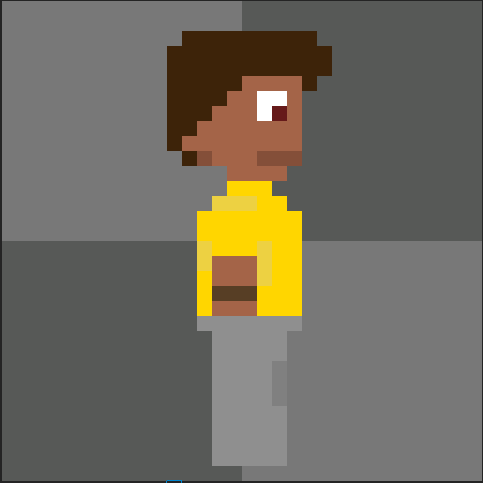
\includegraphics[width=1\linewidth]{figs/pixelLab/dia2/fix_init_1.PNG}
        \caption{\small Sprite do personagem Pablo em um ângulo de 90 graus gerado e editado no Pixel Lab}
        \label{fig:chatGPTPablo90}
    \end{subfigure}
    \begin{subfigure}{0.32\linewidth}
        \centering
        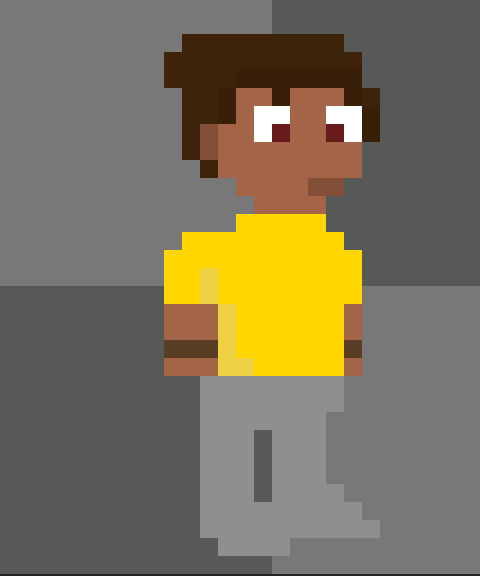
\includegraphics[width=1\linewidth]{figs/pixelLab/dia2/fix_teste_3.PNG}
        \caption{\small Sprite do personagem Pablo em um ângulo de 45 graus gerado e editado no Pixel Lab}
        \label{fig:chatGPTPablo45}
    \end{subfigure}
    \begin{subfigure}{0.32\linewidth}
        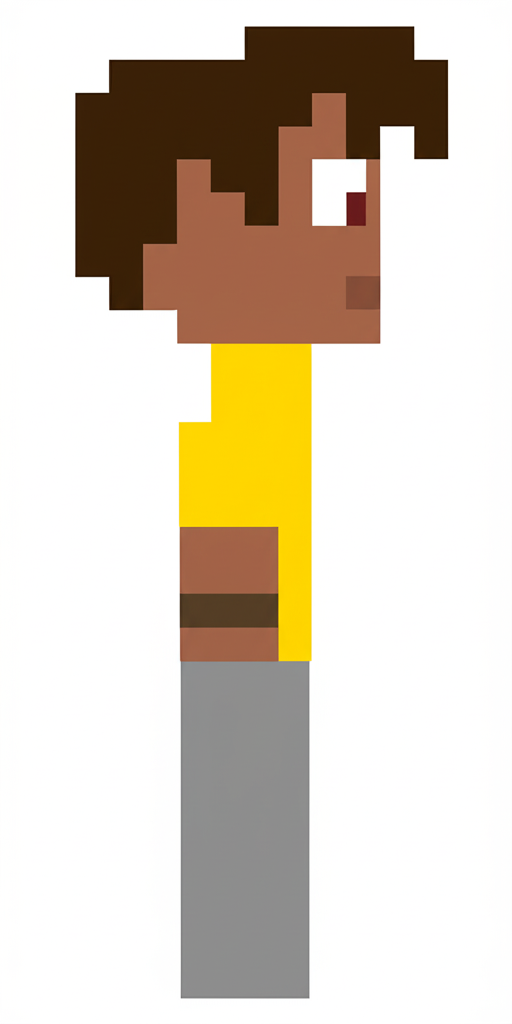
\includegraphics[width=0.7\linewidth]{figs/geminiPro/melhores/chat2_1.png}
        \caption{\small Imagem 1 do personagem Pablo em side view gerada no Gemini Pro}
        \label{fig:chatGPTPabloGeminiPro1}
    \end{subfigure}
    \begin{subfigure}{0.32\linewidth}
        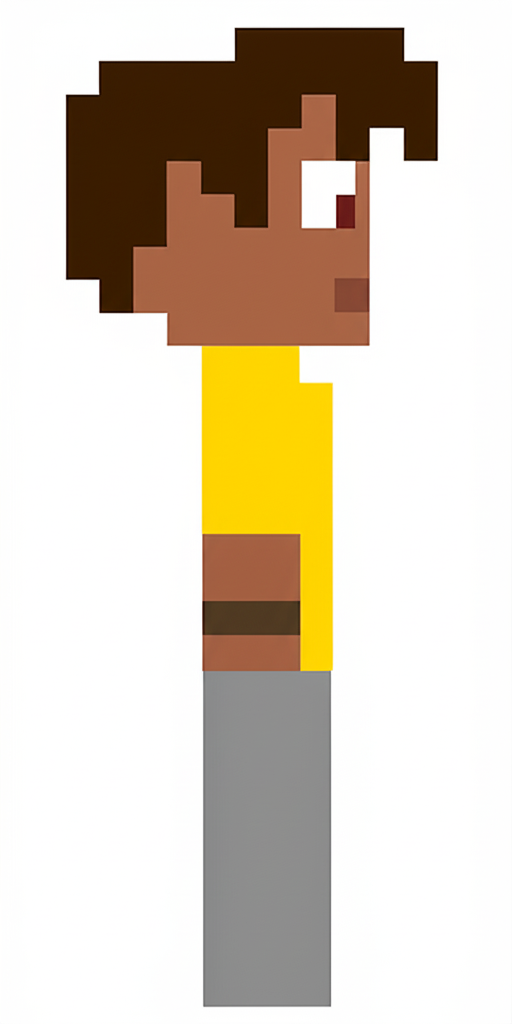
\includegraphics[width=1\linewidth]{figs/geminiPro/melhores/chat2_2.png}
        \caption{\small Imagem 2 do personagem Pablo em side view gerada no Gemini Pro}
        \label{fig:chatGPTPabloGeminiPro2}
    \end{subfigure}
    \begin{subfigure}{0.32\linewidth}
        \centering
        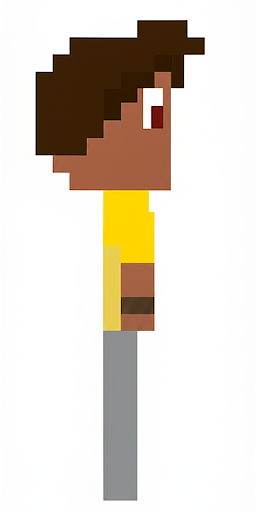
\includegraphics[width=1\linewidth]{figs/geminiPro/melhores/chat5.PNG}
        \caption{\small Imagem 3 do personagem Pablo em side view gerada no Gemini Pro}
        \label{fig:chatGPTPabloGeminiPro3}
    \end{subfigure}
    \legend{\small Fonte: Elaborada pela autora.}
\end{figure}

%   ------------------------------------------------------------------------
\FloatBarrier
\subsection{Geração do sprite em side view}
\label{s.chatGPT.sideview}

Durante os testes iniciais, foi anexada a Figura \ref{fig:chatGPTPablo}, em sua versão de resolução 16x32, com cada pixel da arte realmente valendo um pixel real. Na primeira tentativa, o prompt utilizado instruía a ferramenta a redesenhar o personagem olhando para o lado direito da tela, o que foi interpretado como o personagem apenas com os olhos virados nessa direção em vez do corpo inteiro. Levando esse fator em conta, ainda na mesma interação, o prompt foi reformulado, especificando melhor qual era a posição desejada. Ambos os resultados gerados mantiveram o estilo de pixel art, a consistência das características e tamanho dos pixels, com cores extremamente similares. Apesar disso, o bracelete que o personagem usava não foi gerado, além de ter sido adicionado um sapato cinza escuro, como pode ser visto na Figura \ref{fig:chatGPTSideViewPixel}. Outro detalhe notado foi que o olho ficou ao máximo à direita, sem nenhum pixel do rosto depois dele, priorizando aparentar ao máximo ser pixel perfect em vez de formar uma imagem mais precisa. A interação completa pode ser consultada na Figura \ref{fig:chatGPT1} no Apêndice \ref{ap.telasIA}.

\begin{figure}[htbp]
    \centering
    \caption{\small Imagem em side view gerada pelo ChatGPT }
    \label{fig:chatGPTSideViewPixel}
    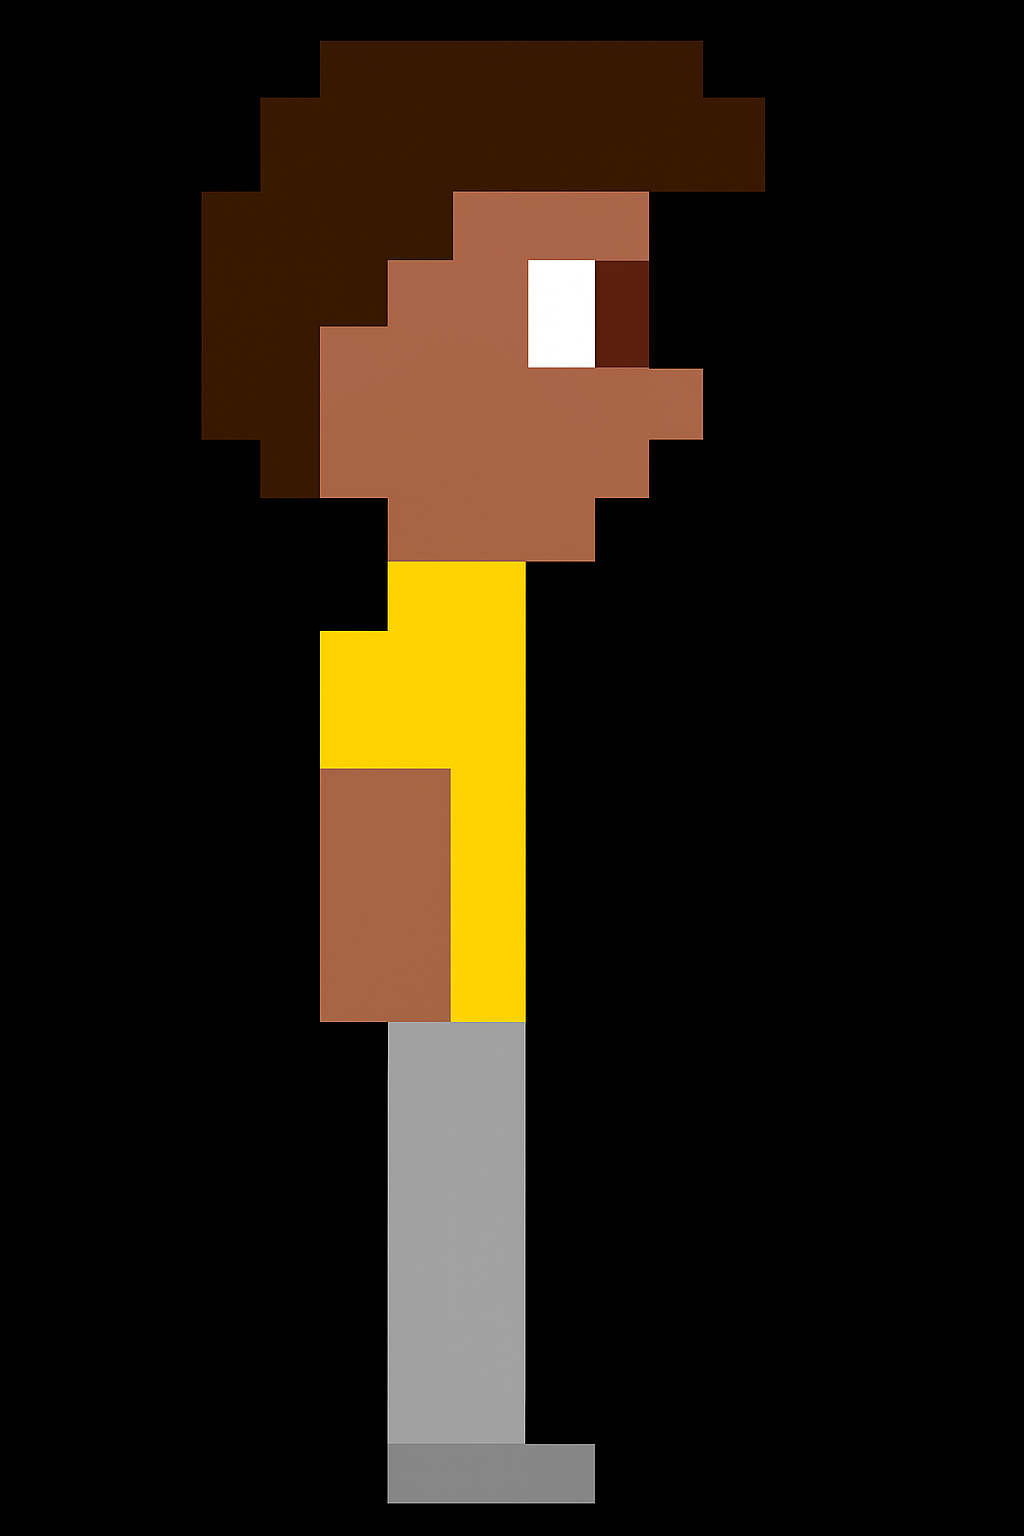
\includegraphics[width=0.3\linewidth]{figs/chatGPT/visao_lateral/res2_pixel.png}
    \legend{\small Fonte: Elaborada pela autora, utilizando a ferramenta ChatGPT.}
\end{figure}

Posteriormente, foi utilizada a mesma imagem de antes, porém em sua versão aumentada, com um prompt textual instruindo a ferramenta a rotacionar o personagem em 90 graus. Além disso, no teste seguinte, também foram anexadas as Figuras \ref{fig:chatGPTPablo90} e \ref{fig:chatGPTPablo45}. Os resultados gerados apresentaram uma melhora na consistência em relação às características, mantendo o bracelete. Porém, foi mais aparente a falta do padrão pixel perfect, além de as imagens formadas apresentarem mais detalhes e tons diferentes, o que resultou em divergências extras com o design original e diferentes formatos de corpo, não tendo uma melhora significativa em comparação com o sprite em side view de referência. O melhor resultado (Figura \ref{fig:chatGPTSideView}) foi gerado antes do anexo dos novos ângulos do personagem para referência, o que indica que as figuras criadas no Pixel Lab diminuíram a performance da geração no ChatGPT. Interação completa demonstrada na Figura \ref{fig:chatGPT2} no Apêndice \ref{ap.telasIA}. 

\begin{figure}[htbp]
    \centering
    \caption{\small Melhor sprite em side view gerado pelo ChatGPT }
    \label{fig:chatGPTSideView}
    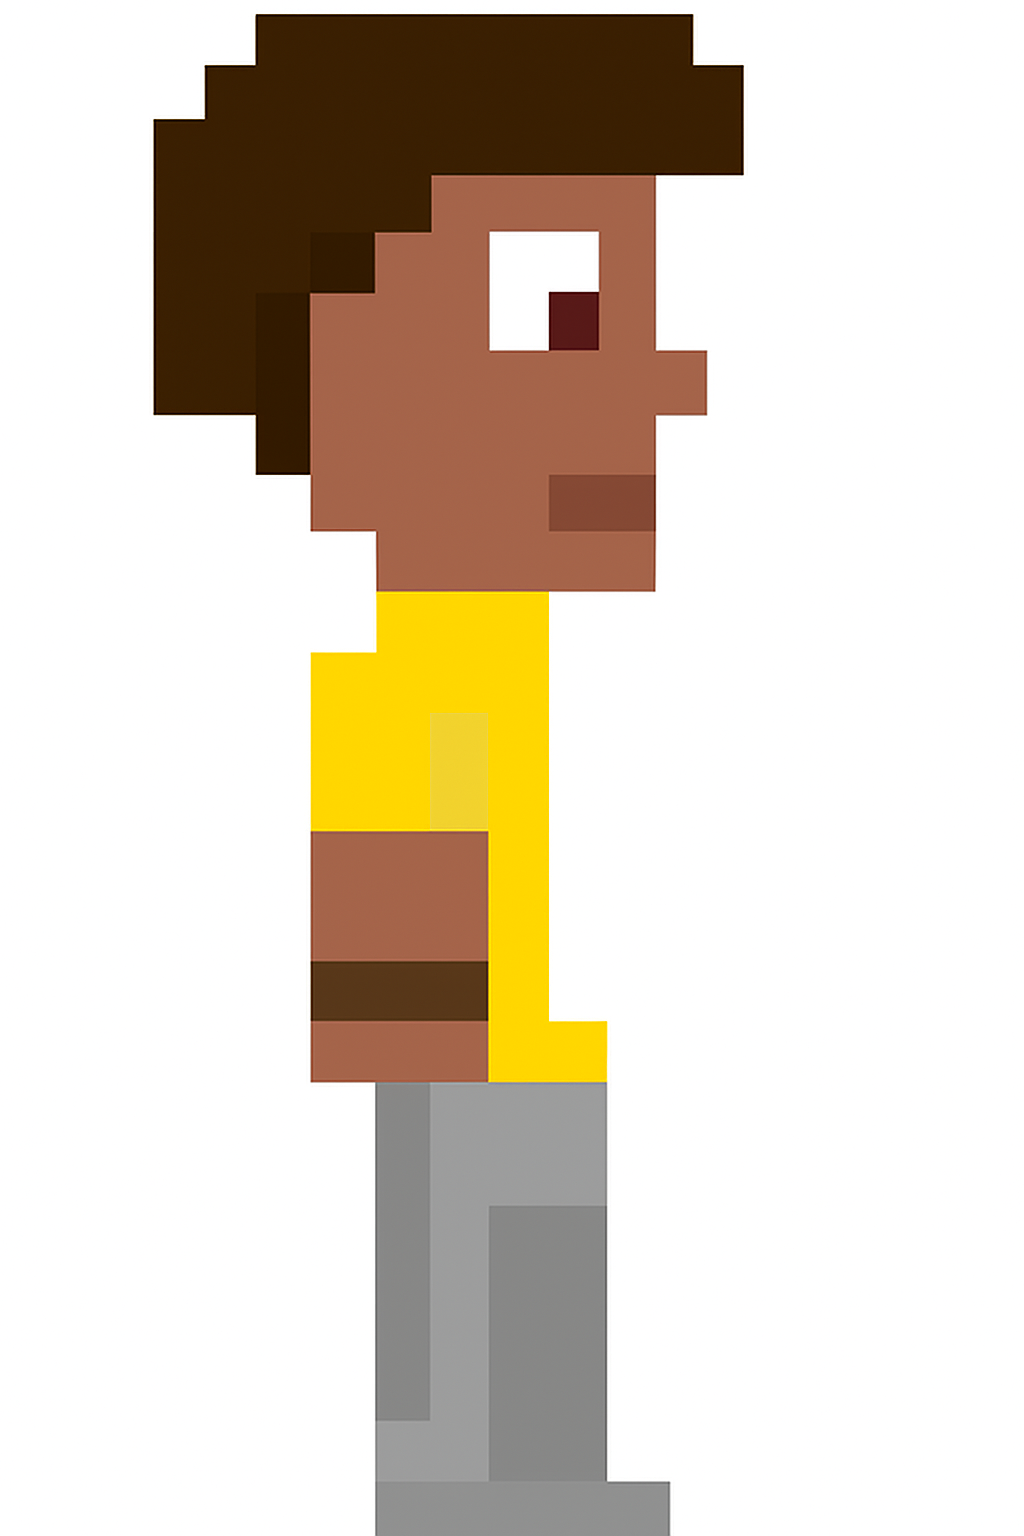
\includegraphics[width=0.3\linewidth]{figs/chatGPT/visao_lateral/res1.png}
    \legend{\small Fonte: Elaborada pela autora, utilizando a ferramenta ChatGPT.}
\end{figure}

Na tentativa subsequente, foi iniciado um novo chat para apontar em detalhes o que cada imagem de referência representava, anexando, além da imagem em front view, os melhores sprites gerados em side view (Figuras \ref{fig:chatGPTPabloGeminiPro1} a \ref{fig:chatGPTPabloGeminiPro3} e Figura \ref{fig:chatGPTSideView}). Também foi incluída para contexto a Figura \ref{fig:chatGPTPablo45}, com o intuito de mostrar um meio termo de resultado satisfatório entre a front view e a side view. Os resultados apresentaram um erro de cropping (recorte, em inglês), onde a parte superior e inferior das imagens ficavam fora da tela, sendo cortadas para fora, uma limitação já conhecida da ferramenta \cite{openaiImage_2025}. Isso pode ser visto na Figura \ref{fig:chatGPTCropping}. Foram testados alguns prompts direcionando a IA a editar a imagem e corrigir a falha, porém não foi efetivo, como pode ser consultado na Figura \ref{fig:chatGPT3} no Apêndice \ref{ap.telasIA}.

\begin{figure}[htbp]
    \centering
    \caption{\small Erro no cropping}
    \label{fig:chatGPTCropping}
    
\includegraphics[width=0.3\linewidth]{figs/chatGPT/visao_lateral/res4.png}
    \legend{\small Fonte: Elaborada pela autora, utilizando a ferramenta ChatGPT.}
\end{figure}

Apesar do ChatGPT não apresentar melhor performance em comparação com as próximas a serem analisadas, é possível notar sua grande capacidade em manter a consistência e o estilo do personagem, sendo extremamente fácil e acessível de usar. Os erros encontrados não tiveram nenhuma relação com a imagem ser em 2D, e não houve grande dificuldade em gerar uma pixel art, apesar de não ser pixel perfect. O melhor sprite gerado nessa fase (Figura \ref{fig:chatGPTSideView}) vai ser usado como referência durante a análise da Ferramenta Gemini Pro (detalhada na Seção \ref{s.ferramentaB}).


%   ------------------------------------------------------------------------
\FloatBarrier
\subsection{Geração do sprite sheet do personagem andando}
\label{s.chatGPT.spriteSheet}

Para a geração do sprite sheet foram utilizadas duas estratégias: a primeira utilizando apenas o sprite de front view como referência e a segunda utilizando mais imagens para a referência.

Os resultados gerados pelo primeiro método foram insatisfatórios. Apesar de, em geral, haver uma consistência entre a referência e a geração, algumas características eram deixadas de lado, e o estilo de pixel art era ou mais complexo ou mais simples. O principal problema encontrado foi o fato de o sprite sheet apresentar apenas um ou dois sprites substancialmente distintos, com o resto deles sendo basicamente repetidos, como pode ser visto na Figura \ref{fig:chatGPTSpriteSheetFront}.

\begin{figure}[htbp]
    \centering
    \caption{\small Sprite sheet com basicamente a mesma etapa do movimento de andar gerado pelo ChatGPT}
    \label{fig:chatGPTSpriteSheetFront}
    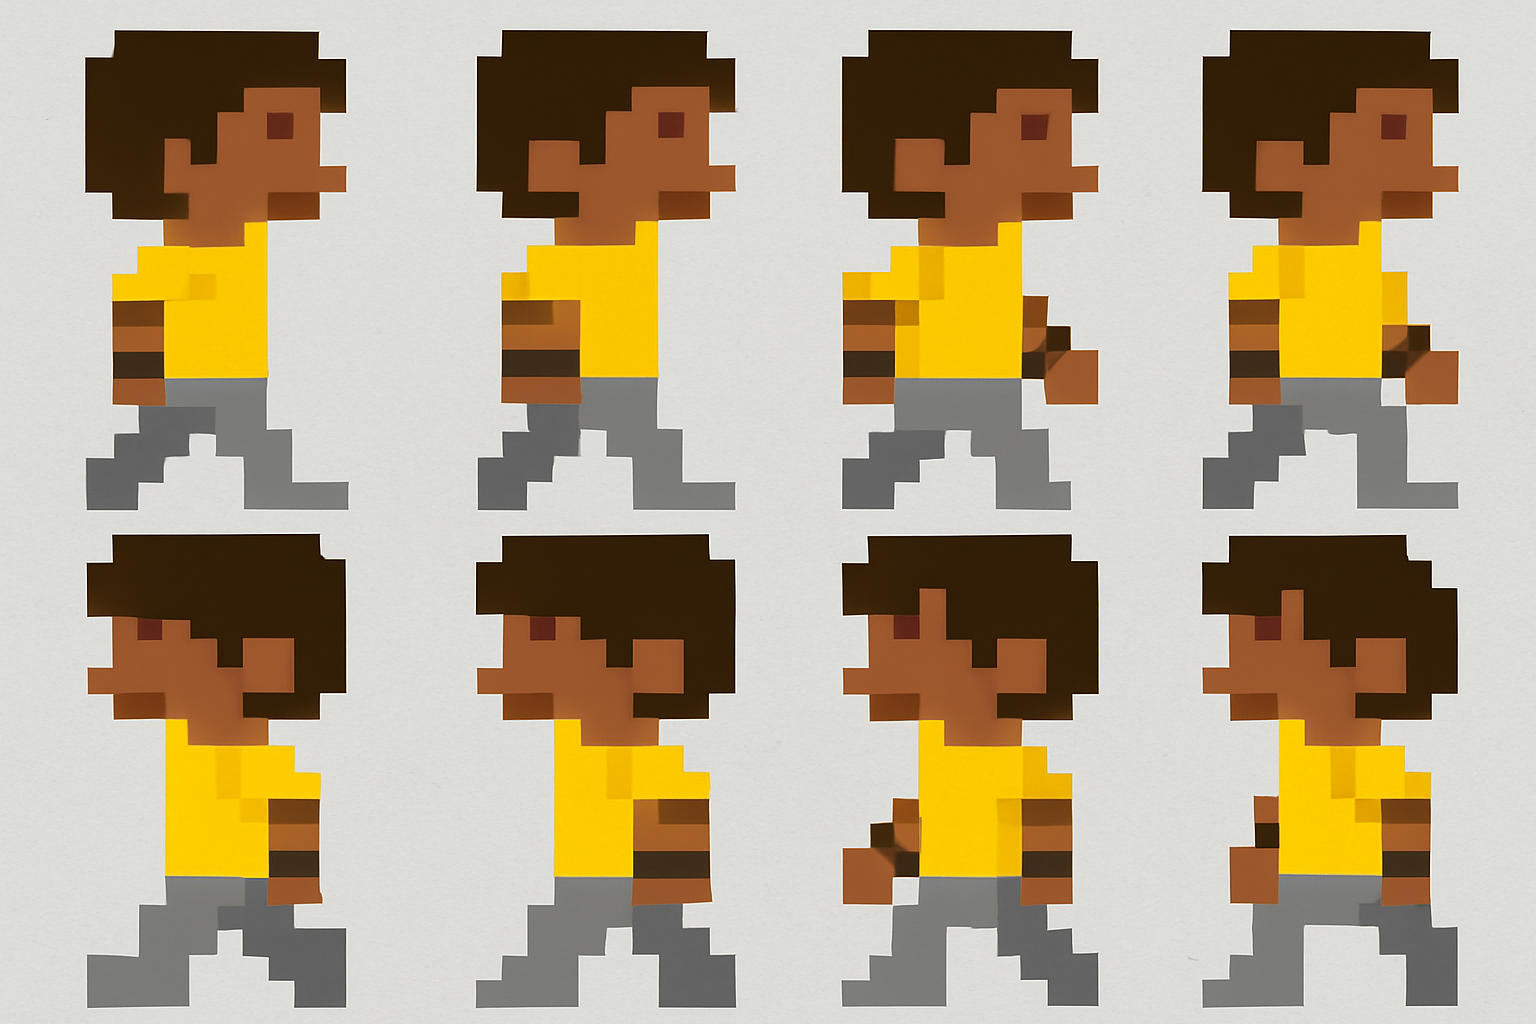
\includegraphics[width=0.6\linewidth]{figs/chatGPT/walking_cycle/front_view/walk cycle 2.png}
    \legend{\small Fonte: Elaborada pela autora, utilizando a ferramenta ChatGPT.}
\end{figure}

Durante a segunda bateria de testes, além de sempre anexar a imagem em front view, no primeiro caso utilizou-se também as imagens geradas pelo Pixel Lab como referência (Figuras \ref{fig:chatGPTPablo90} e \ref{fig:chatGPTPablo45}), enquanto no segundo foi usada como referência a melhor geração do sprite em side view no ChatGPT (Figura \ref{fig:chatGPTSideView}). 

Analisando os resultados, foi notada uma piora na qualidade do produto, com mais deformações nas características, como um terceiro braço ou duas pupilas, e erros em reproduzir a pixel art. Além disso, o sprite sheet ainda é principalmente composto pelo mesmo frame, onde as únicas mudanças não afetam o movimento desejado e apenas alteram a aparência do personagem. Esses detalhes podem ser vistos na Figura \ref{fig:chatGPTSpriteSheetSide}

\begin{figure}[htbp]
    \centering
    \caption{\small Sprite sheet usando a imagem em side view de referência gerado pelo ChatGPT}
    \label{fig:chatGPTSpriteSheetSide}
    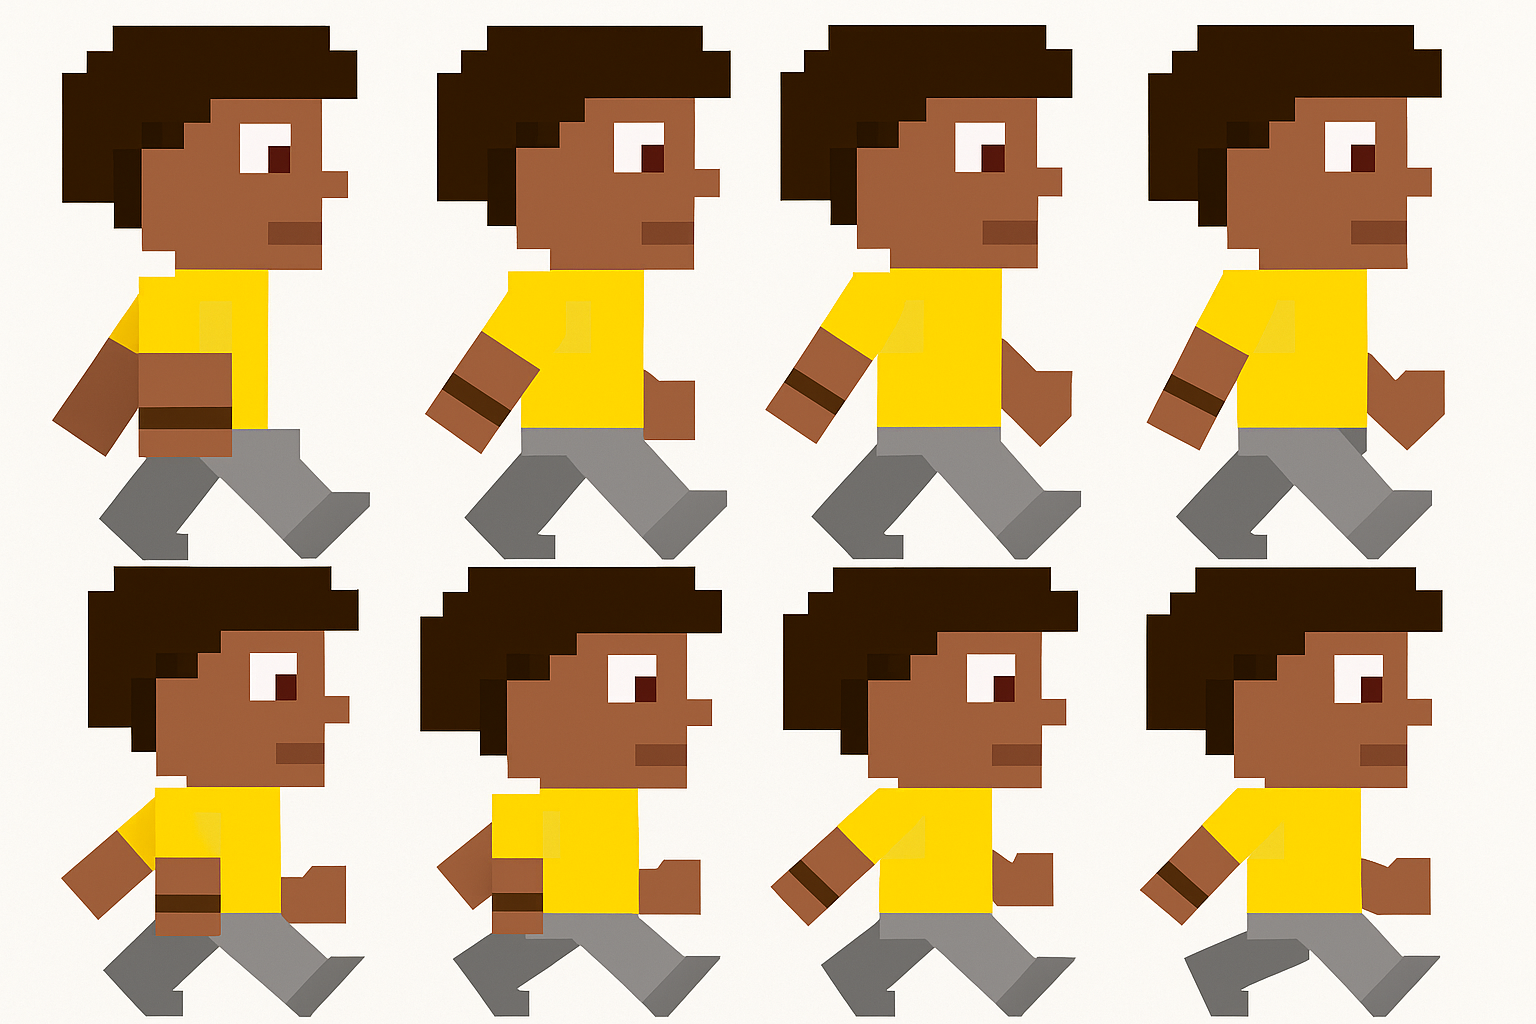
\includegraphics[width=0.6\linewidth]{figs/chatGPT/walking_cycle/side_view/walking cycle 2.png}
    \legend{\small Fonte: Elaborada pela autora, utilizando a ferramenta ChatGPT.}
\end{figure}

Em conclusão, o ChatGPT não mostrou-se adequado para tentar criar um sprite sheet, apresentando mais erros em relação à consistência ao tentar criar esse artefato em relação a apenas criar um sprite específico.